
\documentclass[aspectratio=169,10pt]{beamer}

\usetheme[progressbar=frametitle]{metropolis}
\metroset{numbering=fraction, block=fill}

\usepackage{amsmath, amssymb, bm}
\usepackage{booktabs}
\usepackage{array}
\usepackage{tabularx}
\usepackage{adjustbox}
\usepackage{tikz}
\usetikzlibrary{positioning, arrows.meta, fit, backgrounds, calc, shapes.geometric}

% ── Column types for tables (from v5 variants) ─────────────────────────────
\newcolumntype{L}[1]{>{\raggedright\arraybackslash}p{#1}}
\newcolumntype{C}[1]{>{\centering\arraybackslash}p{#1}}

% ── Math macros reused from the v5 report ──────────────────────────────────
\newcommand{\sg}{\operatorname{sg}}
\newcommand{\cossim}{\operatorname{cos}}
\newcommand{\xhat}{\hat{x}_0}
\newcommand{\xtil}{\tilde{x}_0}
\newcommand{\ftext}{\bar{f}_{\mathrm{text}}}
\newcommand{\fimg}{\bar{f}_{\mathrm{img}}}

% ── Small helpers for the talk ─────────────────────────────────────────────
\newcommand{\litref}[1]{{\scriptsize\color{black!55}[#1]}}
\newcommand{\swatch}[1]{\tikz[baseline=-0.55ex]\node[draw=black!50, fill=#1,
  minimum width=2.6mm, minimum height=2.6mm, inner sep=0pt]{};}
\newcommand{\takeaway}[1]{\vspace{0.25em}$\Rightarrow$ \alert{#1}}

\title[Encoder-Scored Self-Distillation]{Encoder-Scored Self-Distillation
  for Prompt--Image Alignment in Flow-Matching Text-to-Image Models}
\subtitle{Project introduction \& literature review}
\date{\today}

\begin{document}

\maketitle

% ---------------------------------------------------------------------------
\begin{frame}{Talk roadmap}
  \begin{columns}[T]
    \begin{column}{0.48\textwidth}
      \begin{block}{Problem}
        Sampling is slow, and prompt--image alignment is still brittle on
        binding, counting, relations, and multi-object composition.
      \end{block}
      \begin{block}{Prior work}
        Diffusion distillation mostly optimizes \emph{speed}; reward /
        preference tuning optimizes \emph{alignment} but usually pays for
        pixel decoding, reward models, or human preference data.
      \end{block}
    \end{column}
    \begin{column}{0.48\textwidth}
      \begin{alertblock}{Project hypothesis}
        The distillation rollout already gives a small candidate set per
        prompt. Use a cheap latent CLIP proxy to make the loop prefer the
        better-aligned trajectories and timesteps.
      \end{alertblock}
      \begin{block}{Outcome}
        Encoder-scored self-distillation: guided Tweedie consistency targets,
        detached Boltzmann weights, and an explicit latent-space alignment
        reward.
      \end{block}
    \end{column}
  \end{columns}
  \vspace{0.4em}
  {\scriptsize Plan: \textbf{(1)} the distillation problem $\to$
   \textbf{(2)} the prompt--image mismatch $\to$ \textbf{(3)} REPA $\to$
   \textbf{(4--6)} prior work (speed, alignment, closest relatives) $\to$
   \textbf{(7)} positioning $\to$ \textbf{(8)} our method $\to$
   \textbf{(9)} evaluation \& risks $\to$ \textbf{(10)} early results.}
\end{frame}

% ===========================================================================
\section{The distillation problem}
% ===========================================================================

\begin{frame}{Sampling is solving an ODE --- slowly}
  \begin{itemize}
    \item Diffusion / flow-matching sampling numerically integrates the
      probability-flow ODE:
      \[
        z_{k+1} = z_k + (\sigma_{k+1} - \sigma_k)\, v(z_k, t_k, c)
        \qquad \text{(Euler, flow matching)}
      \]
    \item Good quality needs many network evaluations (NFEs); classifier-free
      guidance \emph{doubles} every step (cond.\ $\Vert$ uncond.\ forward).
    \item Better solvers --- DDIM \litref{Song et al., 2021}, DPM-Solver
      \litref{Lu et al., 2022}, EDM-Heun \litref{Karras et al., 2022} ---
      get from hundreds of NFEs to a few dozen \emph{without retraining}, but
      quality degrades sharply below ${\sim}20$ NFEs.
    \item \alert{The distillation problem:} given a pretrained \emph{teacher},
      train a \emph{student} that reaches (almost) the teacher's output in far
      fewer steps.
  \end{itemize}
  \vspace{0.2em}
  \begin{center}
  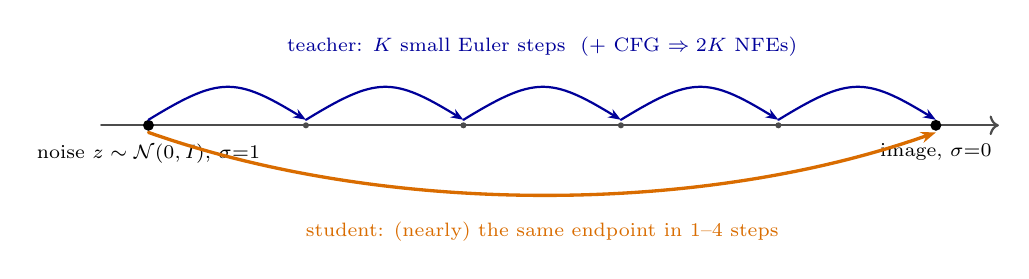
\begin{tikzpicture}[font=\scriptsize, line cap=round]
    \draw[->, thick, black!70] (-0.2,0) -- (11.2,0);
    \node[circle, fill=black, inner sep=1.4pt,
      label={[label distance=1pt]below:{noise $z \sim \mathcal{N}(0, I)$, $\sigma{=}1$}}] (zT) at (0.4,0) {};
    \node[circle, fill=black, inner sep=1.4pt,
      label={[label distance=1pt]below:{image, $\sigma{=}0$}}] (z0) at (10.4,0) {};
    \foreach \x in {2.4,4.4,6.4,8.4} \fill[black!70] (\x,0) circle (1.1pt);
    \foreach \a/\b in {0.4/2.4, 2.4/4.4, 4.4/6.4, 6.4/8.4, 8.4/10.4}
      \draw[-{Stealth[length=1.6mm]}, blue!60!black, thick]
        (\a,0.07) .. controls (\a+0.9,0.62) and (\b-0.9,0.62) .. (\b,0.07);
    \node[blue!60!black] at (5.4,1.0)
      {teacher: $K$ small Euler steps \ ($+$ CFG $\Rightarrow 2K$ NFEs)};
    \draw[-{Stealth[length=1.9mm]}, orange!85!black, very thick]
      (0.4,-0.09) .. controls (3.4,-1.15) and (7.4,-1.15) .. (10.4,-0.09);
    \node[orange!85!black] at (5.4,-1.35)
      {student: (nearly) the same endpoint in $1$--$4$ steps};
  \end{tikzpicture}
  \end{center}
\end{frame}

\begin{frame}{Anatomy of a distillation method}
  Every method in this space picks four things:
  \begin{enumerate}
    \item \textbf{Teacher / target source} --- a frozen pretrained model, a
      progressively re-distilled one, or the student's own EMA
      (\emph{self}-distillation).
    \item \textbf{Matched quantity} --- next state, trajectory endpoint $x_0$,
      an anytime $t \to s$ jump, or the whole output distribution.
    \item \textbf{Metric} --- $\ell_2$, pseudo-Huber, LPIPS, adversarial,
      score-based.
    \item \textbf{Weighting} --- which (trajectory, timestep) pairs count.
      Almost always \emph{uniform}.
  \end{enumerate}
  \vspace{0.6em}
  \begin{alertblock}{Observation}
    Distillation is usually aimed at \emph{speed} --- but its rollouts already
    produce, for free, $N$ candidate generations per prompt with per-timestep
    clean estimates. That structure can be re-aimed at \emph{alignment}: choice
    (4) is the lever this project pulls.
  \end{alertblock}
\end{frame}

\begin{frame}{Project thesis, after reading the literature}
  \begin{columns}[T]
    \begin{column}{0.49\textwidth}
      \textbf{What prior work mostly optimizes}
      \begin{itemize}
        \item \textbf{Fewer NFEs}: distill a many-step sampler into 1--8 steps.
        \item \textbf{Teacher imitation}: match a trajectory point, endpoint,
          flow map, score, or output distribution.
        \item \textbf{Generic quality}: FID / human preference / adversarial
          realism.
      \end{itemize}
    \end{column}
    \begin{column}{0.49\textwidth}
      \textbf{What this project changes}
      \begin{itemize}
        \item Treat teacher rollouts as a \textbf{mini population} of candidate
          prompt completions.
        \item Score candidate \(\hat{x}_0\)'s in \textbf{latent space} against
          the text embedding.
        \item Use the score to \textbf{weight which distillation targets
          matter}, not just to fine-tune after sampling.
      \end{itemize}
    \end{column}
  \end{columns}
  \vspace{0.45em}
  \begin{alertblock}{One-sentence contribution}
    A self-distillation objective for flow-matching T2I models that turns CFG
    rollouts into soft best-of-\(N\) alignment targets using a cheap REPA-style
    CLIP-space latent scorer.
  \end{alertblock}
\end{frame}

% ===========================================================================
\section{The prompt--image mismatch}
% ===========================================================================

\begin{frame}{Images don't always follow prompts}
  \begin{itemize}
    \item Even strong T2I models fail at \textbf{attribute binding}
      (\emph{``a red book and a yellow vase''} $\to$ colors swap or blend),
      \textbf{counting}, \textbf{spatial relations}, and multi-object
      composition. \litref{Huang et al., 2023 --- T2I-CompBench}
    \item Standard measurement:
      $\mathrm{CLIPScore} = \cossim\!\big(\mathrm{CLIP}_{\mathrm{img}}(x),\,
      \mathrm{CLIP}_{\mathrm{text}}(c)\big)$ \litref{Hessel et al., 2021};
      compositional splits (color / shape / texture / spatial / non-spatial /
      complex) in T2I-CompBench; object-focused detection-based protocol in
      GenEval. \litref{Ghosh et al., 2023}
    \item Root cause: pretraining maximizes the likelihood of noisy web
      (image, caption) pairs --- nothing in the objective optimizes prompt
      adherence \emph{directly}.
    \item Concretely on our backbone: SD3.5-M scores only ${\sim}63\%$ on
      GenEval out of the box. \litref{Liu et al., 2025 --- Flow-GRPO}
  \end{itemize}
\end{frame}

\begin{frame}{Existing levers, and what they cost}
  \begin{itemize}
    \item \textbf{CFG at sampling time} \litref{Ho \& Salimans, 2022}:
      raising $\omega$ improves adherence but trades diversity / realism, adds
      $2\times$ NFE, and fixes nothing in the weights.
    \item \textbf{Reward fine-tuning}: ImageReward + ReFL
      \litref{Xu et al., 2023} --- needs a trained reward network, plus a VAE
      decode and a reward forward inside the training loop.
    \item \textbf{Preference optimization}: Diffusion-DPO
      \litref{Wallace et al., 2024} --- needs human preference pairs.
    \item \textbf{Online RL}: Flow-GRPO \litref{Liu et al., 2025} --- needs
      explicit verifier rewards, SDE rollouts, and KL control against reward
      hacking. (Full tour of this family in Part II of the related work.)
  \end{itemize}
  \vspace{0.6em}
  \begin{alertblock}{Our question}
    Can the distillation loop \emph{itself} be re-aimed at prompt--image
    alignment --- with no reward-model network, no preference data, and no
    pixel-space decoding inside the loop?
  \end{alertblock}
\end{frame}

% ===========================================================================
\section{From representation alignment to a latent scorer}
% ===========================================================================

\begin{frame}{REPA: pretrained representations make diffusion training easier}
  \begin{itemize}
    \item \textbf{REPA} \litref{Yu et al., 2025}: regularize the diffusion
      transformer's hidden states toward \emph{frozen} DINOv2 features of the
      clean image, through a small trainable MLP projector
      (cosine-similarity objective).
    \item Effect: ${>}17\times$ faster SiT training and better FID --- semantic
      structure is injected from a self-supervised vision encoder instead of
      being slowly re-learned.
    \item A whole family followed: REPA-E (end-to-end VAE $+$ DiT tuning
      through the REPA loss) \litref{Leng et al., 2025}, U-REPA (U-Nets)
      \litref{Tian et al., 2025}, VideoREPA, HASTE, REG, dispersive loss,
      \dots\ --- and, on the \emph{alignment} side, SoftREPA
      \litref{Lee et al., 2025} (more on this later).
    \item Recipe we keep:
      \begin{itemize}
        \item a \emph{frozen} pretrained encoder defines the feature space;
        \item a \emph{small co-trained projector} (3-layer MLP, hidden 2048)
          bridges into it;
        \item supervision is a cosine alignment in that space.
      \end{itemize}
  \end{itemize}
\end{frame}

\begin{frame}{Our twist: from regularizer to \emph{scorer}}
  \begin{itemize}
    \item Projector $g_\phi$: VAE latents $\to$ \textbf{CLIP joint
      text--image space} ($16 \to 2048 \to 2048 \to 768$ as $1{\times}1$ convs
      $\equiv$ REPA's per-token Linears; parameter-free GroupNorm input norm
      because the scale of $\xhat$ varies with $t$; global mean pool).
    \item Two frozen CLIP ViT-L/14 targets:
      \begin{itemize}
        \item \textbf{text tower}, per step: $\ftext(c)$ --- scoring target,
          $\;s = \cossim(g_\phi(\xhat), \ftext)$ is a \alert{learned CLIPScore
          proxy};
        \item \textbf{image tower}, precomputed once: $\fimg(x_{\mathrm{real}})$
          --- regression anchor $\mathcal{L}_{\mathrm{align}}$ on real COCO
          latents.
      \end{itemize}
    \item The anchor keeps $g_\phi$ a faithful latent-space image encoder, so
      the reward cannot be hacked by collapsing the projector toward the text
      direction.
    \item No VAE decode, no CLIP-vision forward in the training loop --- the
      projector amortizes both.
  \end{itemize}
  \begin{alertblock}{Key difference from REPA}
    REPA regularizes internal representations during model training. We use the
    pretrained representation as an \emph{online scorer} that changes which
    self-distillation targets receive weight.
  \end{alertblock}
\end{frame}

% ===========================================================================
\section{Prior work I: distillation for speed}
% ===========================================================================

\begin{frame}{The landscape in one picture}
  Two broad families \litref{survey: Fan et al., 2025}:
  \vspace{0.2em}
  \begin{columns}[T]
    \begin{column}{0.48\textwidth}
      \textbf{Trajectory distillation}\\[2pt]
      {\small Imitate the teacher's PF-ODE \emph{path} (or jumps along it).
      Needs trajectory data (real or teacher-synthesized); bounded by the
      teacher.}\\[3pt]
      {\footnotesize direct regression $\to$ progressive $\to$ consistency
      (CM / iCT / LCM / PCM / Hyper-SD) $\to$ anytime jumps (CTM, sCM) $\to$
      flow maps (shortcut, MeanFlow, AYF)}
    \end{column}
    \begin{column}{0.48\textwidth}
      \textbf{Score / distribution distillation}\\[2pt]
      {\small Match the student's \emph{output distribution} to the teacher's
      via score functions; can be data-free; can \emph{surpass} the
      teacher.}\\[3pt]
      {\footnotesize SDS / VSD $\to$ Diff-Instruct $\to$ DMD / DMD2 $\to$
      SiD family / $f$-distill $\to$ SiD-DiT; adversarial: ADD / LADD}
    \end{column}
  \end{columns}
  \vspace{0.7em}
  \begin{itemize}
    \item Cross-cutting axes: discrete vs.\ continuous time; with vs.\ without
      real data; frozen vs.\ EMA teacher; uniform vs.\ weighted pairs.
    \item \alert{What we borrow}: consistency structure (trajectory side),
      CFG-mixed targets (guidance distillation), pseudo-Huber metric (iCT),
      and an EMA teacher --- then change the \emph{weighting} from uniform
      to alignment-scored.
  \end{itemize}
\end{frame}

\begin{frame}{Trajectory distillation: regression, then progressive halving}
  \begin{itemize}
    \item \textbf{Direct regression} \litref{Luhman \& Luhman, 2021}: solve
      the teacher's full ODE offline for many noises, regress
      student$(z_T) \to$ endpoint. One-step student, but expensive dataset
      construction and capped by solver error.
    \item \textbf{Progressive Distillation} \litref{Salimans \& Ho, 2022}:
      student (initialized from the teacher) learns to match \emph{two}
      teacher DDIM steps in \emph{one}; then the student becomes the new
      teacher and $N \!\to\! N/2$. Repeating yields $8192 \to 4$-step
      samplers; introduced $v$-prediction.
    \item Cost: multiple distillation \emph{phases}, error compounds across
      phases, and each phase re-fixes the step budget.
    \item \textbf{BOOT} \litref{Gu et al., 2023}: bootstrapped, data-free
      variant predicting the teacher's signal-ODE rollouts.
  \end{itemize}
  \takeaway{the question ``why only match 2 steps?'' is what consistency
  models and flow maps answer --- and our asymmetric gap
  $\Delta \in \{1,\dots,3\}$ sits exactly in this design space (match
  $\Delta$ teacher steps in one student evaluation).}
\end{frame}

\begin{frame}{Distilling guidance; straightening flows}
  \begin{itemize}
    \item \textbf{Guidance distillation} \litref{Meng et al., 2023}: distill
      the \emph{CFG-mixed} prediction
      $v_\varnothing + \omega(v_c - v_\varnothing)$ into a single
      ($\omega$-conditioned) forward --- removes the $2\times$ guidance cost
      and is the standard first stage before step-count distillation.
    \item \textbf{Rectified flow / ReFlow} \litref{Liu et al., 2022}: re-train
      on (noise, image) pairs produced by the teacher's ODE to
      \emph{straighten} trajectories; straighter paths $\Rightarrow$ fewer
      Euler steps; basis of InstaFlow's one-step SD \litref{Liu et al., 2024}
      and of the SD3 / FLUX training paradigm \litref{Esser et al., 2024}.
    \item \textbf{Rectified Diffusion} \litref{Wang et al., 2025}: pair
      \emph{quality}, not path straightness, is what matters --- diffusion
      teachers work as well as flow teachers for ReFlow-style training. All
      these remain bounded by the teacher's sample quality.
  \end{itemize}
  \takeaway{we reuse guidance distillation: our consistency targets are the
  teacher's \emph{guided} Tweedie estimates, so prompt adherence from CFG is
  baked into the student's single conditional forward.}
\end{frame}

\begin{frame}{Consistency models: one jump to the endpoint}
  \begin{itemize}
    \item \textbf{CM / CD} \litref{Song et al., 2023}: learn $f_\theta$ with
      $f_\theta(x_t, t) = f_\theta(x_s, s)$ for any two points on the same
      PF-ODE trajectory, plus the boundary condition
      $f_\theta(x_\delta, \delta) = x_\delta$. Train on \emph{adjacent} pairs:
      online net at $t$, EMA / stop-grad target at the solver-stepped
      $t - \Delta t$. Distillation (teacher solver) or training (Monte-Carlo
      score) variants.
    \item \textbf{iCT} \litref{Song \& Dhariwal, 2024}: teacher-free recipe
      that \emph{removes the EMA target} (stop-grad of the online net),
      adds a curriculum on discretization, lognormal noise sampling, and the
      dimension-scaled \textbf{pseudo-Huber} metric
      $d(a,b) = \sqrt{\lVert a-b \rVert_2^2 + c^2} - c$,
      $c = 0.00054\sqrt{D}$ $\Rightarrow$ \alert{we borrow the metric}.
    \item Known failure mode: one-step quality is great, but naive multi-step
      sampling (noise-injection ping-pong) accumulates error --- analyzed
      formally in AYF \litref{Sabour et al., 2025}.
  \end{itemize}
\end{frame}

\begin{frame}{Consistency at scale: LCM, PCM, Hyper-SD}
  \begin{itemize}
    \item \textbf{LCM} \litref{Luo et al., 2023}: consistency in \emph{latent}
      space on Stable Diffusion; consistency pairs are $k$ solver steps apart
      (the \textbf{skipping step}) from a \emph{CFG-augmented} teacher solve
      with guidance-scale conditioning $\Rightarrow$ \alert{our gap $\Delta$
      plays the skipping-step role}, and our CFG-mixed targets play the
      augmented-solver role. LCM-LoRA makes it a plug-in accelerator.
    \item \textbf{Phased Consistency Models} \litref{Wang et al., 2024}:
      split $[0,T]$ into phases, each with its own consistency map ---
      controls error accumulation and restores CFG / negative-prompt
      controllability that LCM loses.
    \item \textbf{Hyper-SD} \litref{Ren et al., 2024}: trajectory-segmented
      consistency distillation (consistency \emph{within} segments,
      progressively merged), then \emph{human-feedback learning} to repair
      low-step quality, then score distillation for one-step --- an early
      sign that \alert{distillation pipelines want a reward stage}.
  \end{itemize}
\end{frame}

\begin{frame}{Anytime jumps and continuous time: CTM, sCM, rCM}
  \begin{itemize}
    \item \textbf{CTM} \litref{Kim et al., 2024}: train $f_\theta(x_t, t, s)$
      to jump \emph{anywhere-to-anywhere} $t \to s$; compare
      $\hat{x}_{t\to s}$ against a solver-assisted
      $\hat{x}_{t \to u \to s}$ (both pushed to $x_0$ with a stop-grad copy);
      total loss $=$ CTM $+$ score matching $+$ GAN. Exposes whole-trajectory
      structure; enables deterministic multistep $\gamma$-sampling.
    \item \textbf{sCM / TrigFlow} \litref{Lu \& Song, 2025}: continuous-time
      consistency at scale ---
      $x_t = \cos(t)\,x_0 + \sin(t)\,z$ unifies EDM and flow matching;
      JVP-based tangent objective, adaptive weighting; 1.5B models on
      ImageNet $512^2$; 2-step samples within ${\sim}10\%$ of teacher FID.
    \item \textbf{SANA-Sprint} \litref{Chen et al., 2025}: applies sCM to T2I
      --- but must first \emph{fine-tune rectified-flow checkpoints into
      TrigFlow}; chose consistency over DMD partly due to DMD instability.
    \item \textbf{rCM} \litref{Zheng et al., 2025}: sCM's forward-divergence
      objective is mode-covering and accumulates error; adding score
      distillation as a \emph{long-skip regularizer} (reverse divergence)
      fixes detail quality at 10B$+$ scale --- matches DMD2 with better
      diversity, no GAN.
  \end{itemize}
\end{frame}

\begin{frame}{Flow maps: the unifying view}
  Let $\Phi(x, t, s) = x + (t - s)\, u(x, t, s)$ be a learned jump $t \to s$
  with displacement field $u$. \litref{Boffi et al., 2024/2025}
  \begin{itemize}
    \item Validity $=$ \textbf{tangent condition} $u(x,t,t) = v(x,t)$
      \emph{plus one of}: Lagrangian
      ($\partial_s \Phi = u(\Phi, s, s)$), Eulerian
      ($\partial_t \Phi + \nabla_x \Phi\, u(x,t,t) = 0$), or semigroup
      ($\Phi(x,t,s) = \Phi(\Phi(x,t,r), r, s)$) --- each condition yields a
      family of self-distillation losses, with or without a pretrained
      teacher.
    \item \textbf{Shortcut models} \litref{Frans et al., 2025}: semigroup
      instantiation --- one network conditioned on step size $d$, trained so
      one $2d$-jump matches two $d$-jumps (self-consistency) plus a flow-matching
      anchor at $d{=}0$.
    \item \textbf{MeanFlow} \litref{Geng et al., 2025}: Eulerian instantiation
      via the \emph{average velocity}
      $u(x_t, r, t) = \frac{1}{t-r}\int_r^t v(x_\tau, \tau)\, d\tau$ and the
      MeanFlow identity $u = v - (t{-}r)\, \frac{d}{dt}u$ (JVP); from-scratch
      1-NFE FID 3.43 on ImageNet $256^2$.
    \item \textbf{Align Your Flow} \litref{Sabour et al., 2025}: two
      continuous-time flow-map objectives (Eulerian / Lagrangian) that
      generalize sCM and flow matching; proves CMs must degrade with more
      steps while flow maps stay strong at all step counts; adds autoguidance
      $+$ optional adversarial finetune.
    \item Limits: flow maps accelerate \emph{sampling} only; fast
      \emph{likelihoods} need jointly distilling the divergence ODE.
      \litref{Ai et al., 2026 --- F2D2}
  \end{itemize}
\end{frame}

\begin{frame}{Score \& distribution distillation I: from SDS to DMD2}
  \begin{itemize}
    \item \textbf{SDS} \litref{Poole et al., 2023 --- DreamFusion}: optimize a
      generator/scene so its renders score highly under a frozen diffusion
      prior --- the prototype for ``teacher score as a reward''.
      \textbf{VSD} \litref{Wang et al., 2023} fixes SDS's over-saturation by
      also estimating the \emph{generator's} score with a fine-tuned copy.
    \item \textbf{Diff-Instruct} \litref{Luo et al., 2023}: data-free
      distillation minimizing an integral KL between student and teacher
      diffused distributions.
    \item \textbf{DMD} \litref{Yin et al., 2024}: reverse-KL gradient
      $\propto s_{\mathrm{teacher}} - s_{\mathrm{fake}}$ with a co-trained
      ``fake'' score net --- but needs a regression loss on precomputed
      teacher (noise, image) pairs for stability.
    \item \textbf{DMD2} \litref{Yin et al., 2024}: drops the regression loss
      (two-time-scale updates for the fake critic), adds a GAN term on real
      data, and enables few-step students via backward simulation ---
      students \emph{outperform the teacher} (FID 1.28 on ImageNet-64).
  \end{itemize}
\end{frame}

\begin{frame}{Score \& distribution distillation II: SiD, $f$-divergences, adversarial}
  \begin{itemize}
    \item \textbf{Score identity Distillation} \litref{Zhou et al., 2024}:
      data-free \emph{Fisher-divergence} formulation with three score-related
      identities; exponentially fast convergence, outperforms the teacher in
      one step. Extensions: guided / data-free T2I (SiD-LSG, long--short
      guidance), adversarial SiDA, few-step SiD.
      \litref{Zhou et al., 2025a--c}
    \item \textbf{$f$-distill} \litref{Xu et al., 2025}: generalizes the
      divergence family ($f$-divergences); \textbf{Flow Generator Matching}
      \litref{Huang et al., 2024} re-derives SiD-style identities with flow
      quantities instead of scores.
    \item \textbf{Adversarial}: ADD / SDXL-Turbo
      \litref{Sauer et al., 2023} --- DINO-feature discriminator $+$ score
      distillation, real-time 1--4 step SDXL; LADD / SD3-Turbo
      \litref{Sauer et al., 2024} moves the discriminator into latent space
      using teacher features.
    \item Trade-off vs.\ trajectory methods: distribution matching is
      mode-seeking (quality $\uparrow$, diversity risk), GAN terms need real
      data and tuning; consistency is mode-covering (diversity $\uparrow$,
      detail risk) --- hence hybrids (CTM, Hyper-SD, rCM, SiDA).
  \end{itemize}
\end{frame}

\begin{frame}{Spotlight: SiD-DiT --- score distillation meets flow matching}
  \litref{Zhou et al., 2025 --- arXiv:2509.25127}
  \begin{itemize}
    \item \textbf{Claim}: under Gaussian assumptions, diffusion and flow
      matching share the same optimal solutions --- shown via Bayes' rule and
      conditional expectations alone (no ODE/SDE machinery); objectives
      differ only in the \emph{weight-normalized timestep distribution}.
    \item Practical consequence: the teacher's $x_0$-prediction is just
      $f_\phi(x_t,t,c) = x_t - t\, v_\phi(x_t,t,c)$ (Tweedie) --- so
      score-distillation losses transfer to velocity networks
      \emph{out of the box}, with CFG ($\omega{=}4.5$) folded into $f_\phi$.
    \item Distills SANA (RF \emph{and} TrigFlow), SD3-M, SD3.5-M/L, FLUX.1-dev
      (0.6B--12B) into 4-step generators with \emph{one} codebase / config;
      data-free, or data-aided with a DiT-internal discriminator (spatial
      pooling, no new parameters); $w_t = 1{-}t$ weighting.
    \item Matches or beats teachers: SD3.5-M FID 20.92 (SiD$^2_a$), SD3.5-L
      FID 20.57 vs.\ teacher 20.81 vs.\ Turbo 26.11, with equal CLIP.
  \end{itemize}
  \takeaway{licenses our setup: SD3.5-M's velocity field can be treated
  exactly like a diffusion model's $x_0$-predictor --- our guided Tweedie
  targets $\xtil = z_k - \sigma_k v^{\mathrm{cfg}}$ are the same object SiD-DiT
  distills, used here for consistency rather than score matching.}
\end{frame}

% ===========================================================================
\section{Prior work II: alignment, rewards, and selection}
% ===========================================================================

\begin{frame}{Measuring alignment (and what trains the scorers)}
  \begin{itemize}
    \item \textbf{Embedding similarity}: CLIPScore
      \litref{Hessel et al., 2021} --- reference-free
      $\cossim(\mathrm{CLIP_{img}}, \mathrm{CLIP_{text}})$; cheap,
      differentiable, but coarse (compressed cosine range, weak on
      counting/relations).
    \item \textbf{Compositional benchmarks}: T2I-CompBench(++)
      \litref{Huang et al., 2023} (attribute binding, spatial, numeracy);
      GenEval \litref{Ghosh et al., 2023} (detector-verified objects /
      colors / counts / positions); DPG-Bench for dense prompts.
    \item \textbf{Learned human-preference RMs}: ImageReward
      \litref{Xu et al., 2023} (137k expert comparisons), HPSv2
      \litref{Wu et al., 2023}, PickScore \litref{Kirstain et al., 2023} ---
      all are fine-tuned CLIP/BLIP-style towers, i.e.\ \emph{another network
      to host and forward}.
  \end{itemize}
  \vspace{0.4em}
  Our learned proxy $s = \cossim(g_\phi(\xhat), \ftext)$ targets CLIPScore
  (the alignment quantity) directly in latent space; T2I-CompBench prompts are
  used as our held-out qualitative probe.
\end{frame}

\begin{frame}{Reward fine-tuning of the base model}
  \begin{itemize}
    \item \textbf{Differentiable-reward backprop}: ReFL
      \litref{Xu et al., 2023} stops a sampling rollout at a random
      \emph{late} step, one-step-predicts $x_0$, decodes, scores with
      ImageReward, and backprops --- the trick we mirror, minus decode and RM.
      DRaFT \litref{Clark et al., 2024} / AlignProp
      \litref{Prabhudesai et al., 2024} backprop through (truncated)
      sampling chains with LoRA / checkpointing.
    \item \textbf{Policy-gradient RL}: DDPO \litref{Black et al., 2024} and
      DPOK \litref{Fan et al., 2023} treat denoising as an MDP; no
      differentiable reward needed, but high variance and prompt-set scaling
      issues.
    \item \textbf{Preference optimization}: Diffusion-DPO
      \litref{Wallace et al., 2024} adapts DPO via the ELBO to 851k
      Pick-a-Pic pairs (SDXL); D3PO, Diffusion-KTO follow.
    \item \textbf{Shared failure mode}: reward over-optimization / hacking
      --- exploiting RM idiosyncrasies (high-frequency noise, oversaturation)
      --- mitigated by KL terms, early stop, or \emph{proxy} rewards.
      \litref{Clark et al., 2024; Li et al., 2025}
  \end{itemize}
\end{frame}

\begin{frame}{RL on flow matching --- the same backbone, the other route}
  \begin{itemize}
    \item \textbf{Flow-GRPO} \litref{Liu et al., 2025}: first online policy
      gradient RL \emph{for flow matching} --- converts the deterministic ODE
      to a marginal-preserving SDE for exploration, reduces denoising steps
      during training, group-relative advantages (GRPO), KL to stop reward
      hacking. On \alert{SD3.5-M (our backbone)}: GenEval $63\% \to 95\%$,
      text rendering $59\% \to 92\%$.
    \item \textbf{DanceGRPO} \litref{Xue et al., 2025}: one GRPO recipe across
      diffusion \emph{and} rectified flow, T2I/T2V/I2V, five reward models;
      up to $+181\%$ over RL baselines on HPSv2.1 / CLIPScore / GenEval.
    \item Costs: explicit reward models or verifiers, on-policy SDE sampling
      ($N$ full rollouts per update \emph{just for the reward}), KL
      bookkeeping.
  \end{itemize}
  \vspace{0.4em}
  Shared skeleton with us: \emph{group of $N$ rollouts per prompt, advantages
  normalized within the group} --- our z-scored Boltzmann weights are the
  distillation-side analogue of GRPO's group-relative advantages, but the
  reward is a co-trained encoder proxy and the update is a weighted
  consistency regression, not a policy gradient.
\end{frame}

\begin{frame}{Selection instead of gradients: best-of-$N$ and its distillation}
  \begin{itemize}
    \item \textbf{Best-of-$N$ at inference}: searching over sampling noises
      with a verifier keeps improving generation quality long after
      denoising-step gains plateau \litref{Ma et al., 2025} --- but the
      $N\times$ cost is paid at \emph{every} generation.
    \item \textbf{Reward-weighted regression / ranked fine-tuning}: RWR
      \litref{Peters \& Schaal, 2007} --- Boltzmann re-weighting
      $w \propto e^{r/\tau}$ of imitation targets; RAFT
      \litref{Dong et al., 2023} --- fine-tune only on top-ranked samples;
      both amortize selection into the weights.
    \item \textbf{BOND} \litref{Sessa et al., 2024}: distill the
      \emph{best-of-$N$ distribution} itself into an LLM policy (Jeffreys
      divergence); the practical J-BOND iterates against a
      \emph{moving EMA anchor} --- structurally, soft best-of-$N$
      self-distillation.
  \end{itemize}
  \takeaway{our reading: a distillation loop already pays for $N$ rollouts;
  scoring them and re-weighting the consistency targets turns the same compute
  into amortized best-of-$N$ --- per trajectory \emph{and} per timestep ---
  with the EMA teacher as the moving anchor.}
\end{frame}

% ===========================================================================
\section{Closest relatives: reward-aware distillation}
% ===========================================================================

\begin{frame}{Rewards inside the distillation loop}
  \begin{itemize}
    \item \textbf{RG-LCD} \litref{Li et al., 2025}: LCM distillation $+$
      maximize a differentiable RM on the single-step generation that the CD
      loss already computes; 2-step student preferred over the 50-step
      teacher. Direct RM gradients cause \emph{high-frequency noise}
      (over-optimization) $\Rightarrow$ they insert a \textbf{latent proxy
      RM}, fine-tuned each iteration to mimic the expert RM.
    \item \textbf{T2V-Turbo (v1/v2)} \litref{Li et al., 2024/2025}: same
      recipe for video --- a \emph{mixture} of image-text and video-text RMs
      scored on the CD single-step generations, bypassing backprop through
      the sampler; v2 adds dataset / guidance design, SOTA VBench.
    \item \textbf{Hyper-SD} \litref{Ren et al., 2024}: dedicated
      human-feedback stage to repair the low-step regime.
    \item \textbf{Diff-Instruct++} \litref{Luo, 2024}: RLHF for one-step
      generators (reward $+$ integral-KL to the teacher); proves
      \alert{CFG-weighted distillation is implicit RLHF} --- theoretical
      support for our guided-Tweedie targets carrying alignment.
  \end{itemize}
\end{frame}

\begin{frame}{SoftREPA: the REPA route to alignment}
  \litref{Lee et al., 2025 --- arXiv:2503.08250}
  \begin{itemize}
    \item Diagnosis: training only on \emph{positive} (image, text) pairs is
      suboptimal representation alignment; T2I models retain residual
      text--image misalignment.
    \item Fix: lightweight \emph{contrastive} fine-tuning --- learnable soft
      text tokens (${<}1$M params) trained with denoising-score-matching
      logits over positive \emph{and negative} pairs; provably increases
      text--image mutual information; works on SD3-class models.
    \item Shared DNA with us: both treat alignment as a
      \emph{representation-space} problem in the REPA tradition, both add
      ${\ll}1\%$ trainable parameters, neither needs preference data.
    \item Key difference: SoftREPA reshapes the \emph{conditioning} (soft
      tokens, contrastive logits); we reshape the \emph{training signal}
      (scored, re-weighted distillation targets $+$ an explicit reward
      through a latent scorer) --- and we get few-step behavior from the
      consistency structure as a side effect.
  \end{itemize}
\end{frame}

\begin{frame}{How we differ from the closest relatives}
  \begin{itemize}
    \item \textbf{Reward source}: RG-LCD / T2V-Turbo / Hyper-SD / DI++ all
      require a pretrained \emph{human-preference RM} (ImageReward, HPS,
      \dots). Our scorer is a 3-layer projector anchored to \emph{frozen CLIP
      image embeddings of real data} --- no preference data, no RM network;
      the ``expert'' is CLIP's joint space itself.
    \item \textbf{Where the reward acts}: they add a reward term
      \emph{next to} a uniform distillation loss. We \emph{additionally}
      re-weight the consistency loss itself --- a detached, z-scored
      Boltzmann $W$ over (trajectory $\times$ timestep) = soft best-of-$N$
      target selection; the reward path
      ($\mathcal{L}_{\mathrm{reward}}$) is deliberately the only
      gradient route for $s$.
    \item \textbf{Reward locus}: their RMs need decoded \emph{pixels} (or a
      proxy distilled from a pixel RM); our proxy reads VAE \emph{latents} of
      Tweedie estimates directly --- zero decode cost at every scored pair.
    \item \textbf{Teacher}: theirs is a frozen external teacher; ours is the
      student's own EMA (self-distillation), so alignment gains compound into
      future targets --- with drift monitored, since nothing external pins
      the loop.
    \item \textbf{Backbone}: first (to our knowledge) reward-aware
      consistency-style loop on a \emph{flow-matching MMDiT} (SD3.5-M) ---
      the regime SiD-DiT showed is safe for diffusion-style distillation.
  \end{itemize}
\end{frame}

\begin{frame}{How this project differs --- at a glance}
  \scriptsize
  \begin{adjustbox}{max width=\textwidth, max height=0.74\textheight, center}
  \begin{tabular}{@{}L{0.23\textwidth}C{0.16\textwidth}C{0.15\textwidth}C{0.15\textwidth}L{0.21\textwidth}@{}}
    \toprule
    \textbf{Question} & \textbf{Consistency / LCM} & \textbf{Flow-map papers} & \textbf{Reward / DPO} & \textbf{Encoder-scored self-distillation} \\
    \midrule
    What is optimized directly? & Endpoint agreement & Jump-map accuracy / fidelity & Human or learned reward & Endpoint agreement \emph{weighted} by latent prompt score \\
    Is the teacher external? & Usually frozen pretrained & Frozen teacher, direct training, or self-distill & Often no teacher; reward/preference source & EMA of the student $+$ guided rollout \\
    Where is the alignment signal computed? & Indirectly via CFG teacher & Indirectly via teacher / autoguidance & Pixel-space reward or preference pairs & Latent projector into CLIP joint space \\
    Are candidate rollouts compared? & Usually no, uniform pairs & Usually no, objective-level pairs & Often pairwise but external / offline & Yes: soft best-of-$N$ over trajectories \& timesteps \\
    Extra runtime inside training loop? & Teacher forwards & Teacher / flow-map forwards & Decode $+$ reward / preference model & No decode; no CLIP image forward; small projector only \\
    \bottomrule
  \end{tabular}
  \end{adjustbox}
  \begin{alertblock}{Thesis in one sentence}
    Distillation rollouts can be treated as an online, prompt-conditioned
    candidate set; a latent CLIP proxy turns uniform consistency training into
    alignment-aware reward-weighted regression.
  \end{alertblock}
\end{frame}

\begin{frame}{Most related papers, ranked by proximity}
  \scriptsize
  \begin{adjustbox}{max width=\textwidth, max height=0.80\textheight, center}
  \begin{tabular}{@{}C{0.045\textwidth}L{0.22\textwidth}L{0.34\textwidth}L{0.34\textwidth}@{}}
    \toprule
    \textbf{\#} & \textbf{Paper} & \textbf{What we reuse / overlap} & \textbf{Critical difference} \\
    \midrule
    1 & SiD-DiT \litref{Zhou et al., 2025} & Score distillation transfers to SD3/SD3.5/FLUX flow-matching DiTs; guided Tweedie as $x_0$-predictor & Score-identity acceleration, \emph{not} prompt-specific encoder-scored target weighting \\
    2 & LCM / LCM-LoRA \litref{Luo et al., 2023} & Guided latent consistency; skipping-step $=$ our $\Delta$; few-step T2I template & Uniform targets; speed objective, no online latent scorer \\
    3 & Align Your Flow \litref{Sabour et al., 2025} & Continuous-time flow maps; arbitrary $t\!\to\!s$ jumps; CMs degrade with steps & Learns general flow maps; our jump target is \emph{selected} by prompt alignment \\
    4 & SD3.5-Flash \litref{Bandyopadhyay et al., 2025} & SD3.5 rectified-flow distillation; split-timestep finetuning for prompt alignment & Public few-step \emph{system}; no latent CLIP weighting of consistency targets \\
    5 & CTM / sCM \litref{Kim et al., 2024; Lu \& Song, 2025} & Anytime $t\!\to\!s$ transitions; JVP tangent objective & No encoder score deciding which trajectories / timesteps matter \\
    6 & REPA \litref{Yu et al., 2025} & Frozen encoder $+$ small projector $+$ cosine alignment & Regularizes hidden states; ours uses the projector as a differentiable \emph{scorer} \\
    7 & RG-LCD / T2V-Turbo \litref{Li et al., 2024/2025} & Reward on the CD single-step generation; latent proxy RM & Needs a pretrained pixel/preference RM; ours anchors to CLIP image features only \\
    8 & ImageReward/ReFL, Diffusion-DPO \litref{Xu 2023; Wallace 2024} & Explicit alignment optimization & Reward model / preference data $+$ pixel scoring; not self-distillation target selection \\
    \bottomrule
  \end{tabular}
  \end{adjustbox}
\end{frame}

% ===========================================================================
\section{Positioning: the gap we target}
% ===========================================================================

\begin{frame}{The gap we target}
  Across the families just toured:
  \begin{enumerate}
    \item \textbf{Distillation} methods (PD, CM/LCM/CTM, flow maps, DMD/SiD)
      weight (trajectory, timestep) pairs \emph{uniformly} --- nobody asks
      \emph{which} rollouts deserve to be matched.
    \item \textbf{Alignment} methods (ReFL, DPO, GRPO, RG-LCD, DI++) buy
      adherence with external machinery: reward networks, preference pairs,
      pixel decodes, or on-policy RL infrastructure.
    \item \textbf{Self-distillation} with an EMA teacher is standard
      \emph{inside} CM training, and EMA anchors appear in LLM alignment
      (J-BOND) --- but an EMA-teacher loop whose targets are
      \emph{selected by a learned alignment score} has not been explored for
      T2I flow matching.
  \end{enumerate}
  \vspace{0.4em}
  \begin{alertblock}{Hypothesis}
    Encoder-scored re-weighting of an asymmetric consistency loss can move
    prompt alignment with \emph{no} reward network, \emph{no} preference
    data, and \emph{no} decode --- at the price of one co-trained projector
    and the rollouts the distillation loop already runs.
  \end{alertblock}
\end{frame}

\begin{frame}{Where our method sits}
  \begin{center}
  \begin{adjustbox}{max width=\textwidth}
  \scriptsize
  \begin{tabular}{@{}lllll@{}}
    \toprule
    \textbf{Method} & \textbf{Teacher} & \textbf{Matched target} & \textbf{Alignment signal} & \textbf{Aim} \\
    \midrule
    Progressive Distillation & frozen, re-distilled per stage & 2 teacher steps $\to$ 1 & --- & speed \\
    CD / iCT / LCM & frozen ($\pm$ EMA / sg target) & endpoint along the ODE & --- & speed \\
    CTM / sCM / flow maps & frozen / none & anytime $t \to s$ jump & --- & speed \\
    DMD2 / SiD / SiD-DiT & frozen score network & output distribution & (GAN on real data) & speed $+$ fidelity \\
    ADD / LADD & frozen $+$ discriminator & realism of samples & --- & speed $+$ fidelity \\
    ReFL / DRaFT / DPO & --- & reward / preference signal & pixel RM / human pairs & alignment \\
    Flow-GRPO / DanceGRPO & --- (policy itself) & group-relative advantage & verifiers / RMs & alignment \\
    RG-LCD / T2V-Turbo & frozen (LCD) & endpoint $+$ RM reward & pixel RM ($+$ latent proxy) & speed $+$ alignment \\
    Hyper-SD & frozen, segmented & segment consistency & human-feedback stage & speed $+$ alignment \\
    Diff-Instruct++ & frozen (IKL reference) & output distribution & pixel RM & alignment (1-step) \\
    SoftREPA & --- (frozen base) & contrastive DSM logits & pos./neg.\ text pairs & alignment \\
    \midrule
    \textbf{Ours} & \textbf{EMA of the student} &
      \textbf{$s$-weighted guided Tweedie $\xtil$} &
      \textbf{latent CLIP proxy (no RM)} & \textbf{alignment} \\
    \bottomrule
  \end{tabular}
  \end{adjustbox}
  \end{center}
  \vspace{0.5em}
  \begin{itemize}
    \item Self-distillation: no external teacher; the EMA \emph{is} the
      teacher, so improvements feed back into future targets.
    \item Asymmetric timestep gap gives the consistency structure; an
      encoder-based score decides \emph{which} targets matter.
  \end{itemize}
\end{frame}

% ===========================================================================
\section{Our method: encoder-scored self-distillation}
% ===========================================================================

\begin{frame}{Method in one slide}
  \begin{itemize}
    \item \textbf{Base}: SD3.5-Medium (2.5B MMDiT, flow matching) at $512^2$;
      VAE latents $16 \times 64 \times 64$.
    \item \textbf{Student} $v_\theta$ trainable; \textbf{teacher}
      $v_\xi = $ fp32 EMA, $\;\xi \leftarrow m\,\xi + (1{-}m)\,\theta$,
      $m = 0.999$ --- \emph{self}-distillation, no external teacher.
    \item \textbf{Pass 1} (no grad): $N{=}4$ CFG rollouts ($\omega{=}7$),
      $K{=}8$ Euler steps; cache \emph{guided} Tweedie targets $\xtil$ on the
      scoring window $k \in \{3, \dots, 7\}$.
    \item \textbf{Pass 2} (one batched forward): student at the \emph{noisier}
      state $z_{k-\Delta}$, $\Delta \sim \mathcal{U}\{1, \dots, 3\}$
      $\Rightarrow$ $\xhat$.
    \item \textbf{Scoring}: REPA-style projector $\to$ CLIP space; detached
      Boltzmann weights over (trajectory $\times$ step) $+$ explicit reward.
    \item \textbf{Not used}: standard diffusion loss; reward-model network.
      Real images only anchor the projector.
  \end{itemize}
\end{frame}

\begin{frame}{All components}
  \begin{center}
  \begin{adjustbox}{max width=\textwidth, max height=0.72\textheight, center}
  % ── Diagram reused from the v5 report (self_distill_v5.tex) ──────────────
  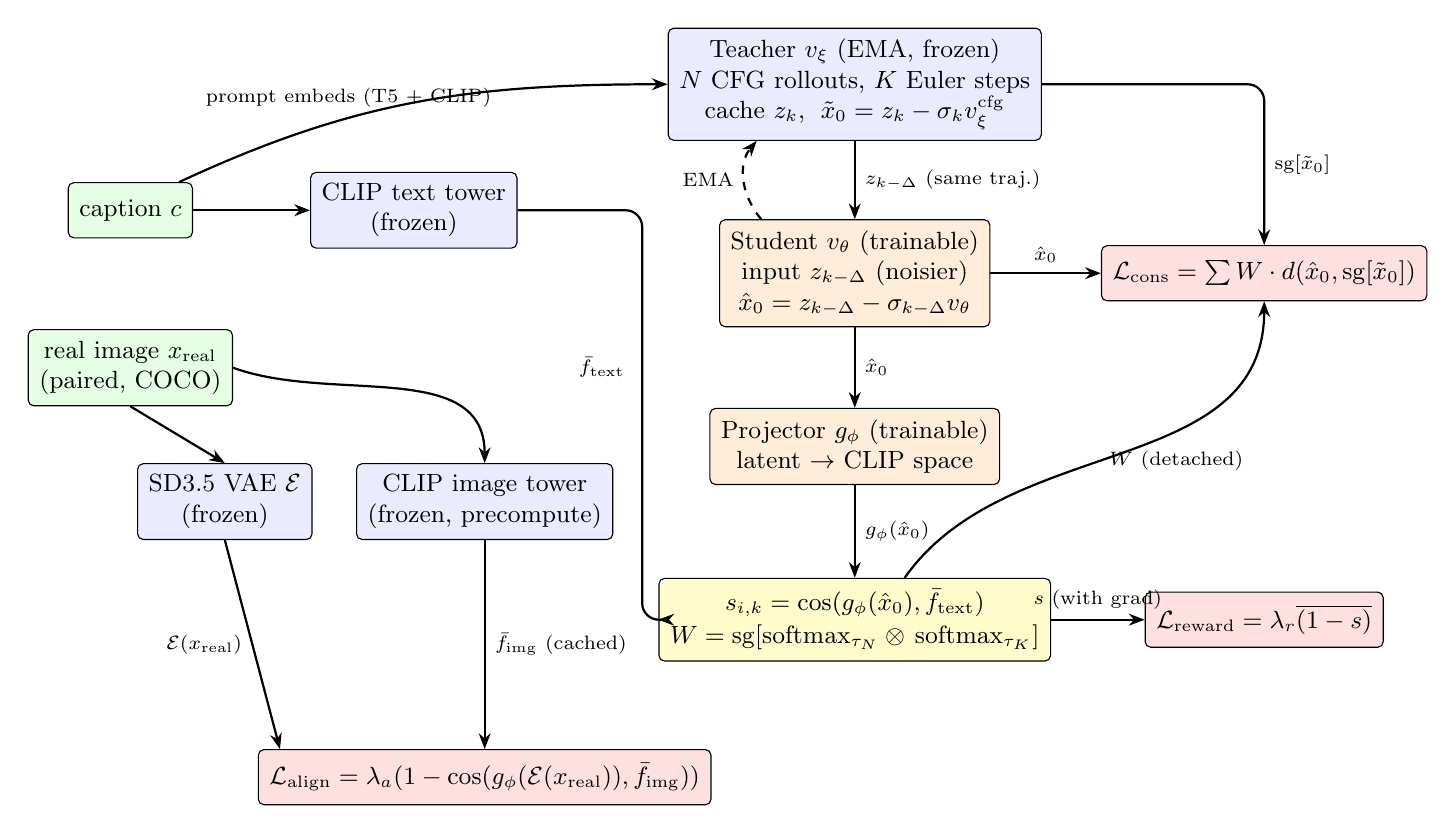
\begin{tikzpicture}[
    font=\small,
    box/.style={draw, rounded corners=2pt, align=center, inner sep=4pt, minimum height=7mm},
    frozen/.style={box, fill=blue!8},
    train/.style={box, fill=orange!15},
    data/.style={box, fill=green!10},
    loss/.style={box, fill=red!12},
    scorebox/.style={box, fill=yellow!20},
    arr/.style={-{Stealth[length=2mm]}, thick},
    dashedarr/.style={arr, dashed},
    lab/.style={font=\scriptsize},
  ]

  % ── Center chain: teacher -> student -> projector -> score ──
  \node[frozen] (teacher) at (9.2, 7.2)
    {Teacher $v_\xi$ (EMA, frozen)\\$N$ CFG rollouts, $K$ Euler steps\\
     cache $z_k$,\; $\xtil = z_k - \sigma_k v^{\mathrm{cfg}}_\xi$};
  \node[train] (student) at (9.2, 4.8)
    {Student $v_\theta$ (trainable)\\input $z_{k-\Delta}$ (noisier)\\
     $\xhat = z_{k-\Delta} - \sigma_{k-\Delta} v_\theta$};
  \node[train] (proj) at (9.2, 2.6)
    {Projector $g_\phi$ (trainable)\\latent $\to$ CLIP space};
  \node[scorebox] (score) at (9.2, 0.4)
    {$s_{i,k} = \cossim(g_\phi(\xhat), \ftext)$\\[1pt]
     $W = \sg[\mathrm{softmax}_{\tau_N} \otimes\, \mathrm{softmax}_{\tau_K}]$};

  % ── Left column: inputs and frozen encoders ──
  \node[data] (caption) at (0, 5.6) {caption $c$};
  \node[frozen] (cliptext) at (3.6, 5.6) {CLIP text tower\\(frozen)};
  \node[data] (image) at (0, 3.6) {real image $x_{\mathrm{real}}$\\(paired, COCO)};
  \node[frozen] (vae) at (1.2, 1.9) {SD3.5 VAE $\mathcal{E}$\\(frozen)};
  \node[frozen] (clipimg) at (4.5, 1.9) {CLIP image tower\\(frozen, precompute)};

  % ── Right column: losses ──
  \node[loss] (lcons) at (14.4, 4.8)
    {$\mathcal{L}_{\mathrm{cons}} = \sum W \cdot d(\xhat, \sg[\xtil])$};
  \node[loss] (lreward) at (14.4, 0.4)
    {$\mathcal{L}_{\mathrm{reward}} = \lambda_r \overline{(1-s)}$};
  \node[loss] (lalign) at (4.5, -1.6)
    {$\mathcal{L}_{\mathrm{align}} = \lambda_a (1 - \cossim(g_\phi(\mathcal{E}(x_{\mathrm{real}})), \fimg))$};

  % ── Center chain edges ──
  \draw[arr] (teacher) -- node[right, lab] {$z_{k-\Delta}$ (same traj.)} (student);
  \draw[arr] (student) -- node[right, lab] {$\xhat$} (proj);
  \draw[arr] (proj) -- node[right, lab] {$g_\phi(\xhat)$} (score);
  \draw[dashedarr] (student.150) to[out=130, in=230]
    node[left, lab] {EMA} (teacher.210);

  % ── Caption conditioning ──
  \draw[arr] (caption) -- (cliptext);
  \draw[arr] (caption.30) to[out=25, in=180]
    node[above, lab, pos=0.35] {prompt embeds (T5 + CLIP)} (teacher.west);
  % f_text wire: down the empty corridor between encoder and center columns
  \draw[arr, rounded corners=6pt]
    (cliptext.east) -- (6.5, 5.6) -- (6.5, 0.4) -- (score.west);
  \node[lab, left] at (6.4, 3.6) {$\ftext$};

  % ── Losses: consistency ──
  \draw[arr] (student.east) -- node[above, lab] {$\xhat$} (lcons.west);
  \draw[arr, rounded corners=6pt] (teacher.east) -|
    node[right, lab, pos=0.75] {$\sg[\xtil]$} (lcons.north);
  \draw[arr] (score.40) to[out=55, in=270]
    node[right, lab, pos=0.45] {$W$ (detached)} (lcons.south);

  % ── Losses: reward ──
  \draw[arr] (score.east) -- node[above, lab] {$s$ (with grad)} (lreward.west);

  % ── Losses: projector anchor ──
  \draw[arr] (image.south) -- (vae.north);
  \draw[arr] (image.east) to[out=-20, in=90] (clipimg.north);
  \draw[arr] (vae.south) -- node[left, lab] {$\mathcal{E}(x_{\mathrm{real}})$}
    ($(lalign.north)+(-2.6,0)$);
  \draw[arr] (clipimg.south) -- node[right, lab] {$\fimg$ (cached)}
    (lalign.north);

  \end{tikzpicture}
  \end{adjustbox}
  \end{center}
  \vspace{0.2em}
  \centering\scriptsize
  \swatch{green!10}~data \quad \swatch{blue!8}~frozen \quad
  \swatch{orange!15}~trainable \quad \swatch{yellow!20}~scoring \quad
  \swatch{red!12}~losses \quad
  dashed arrow $=$ EMA closes the self-distillation loop
\end{frame}

\begin{frame}{Pass 1 --- teacher rollout (no grad)}
  For one caption $c$ per step, the teacher generates $N$ trajectories from
  Gaussian noise with $K$ Euler steps under CFG:
  \[
    v^{\mathrm{cfg}}_\xi = v_\xi(z_k, t_k, \varnothing)
      + \omega \big( v_\xi(z_k, t_k, c) - v_\xi(z_k, t_k, \varnothing) \big),
    \qquad
    z_{k+1} = z_k + (\sigma_{k+1} - \sigma_k)\, v^{\mathrm{cfg}}_\xi
  \]
  At every $k$ in the scoring window
  $\mathcal{K} = \{ \lceil 0.4K \rceil, \dots, \lfloor 0.9K \rfloor \}$, cache
  the teacher's Tweedie estimate from the \emph{CFG-mixed} velocity:
  \[
    \xtil^{(i,k)} = z^{(i)}_k - \sigma_k\,
      v^{\mathrm{cfg}}_\xi\big(z^{(i)}_k, t_k, c\big)
  \]
  \begin{itemize}
    \item Mid-to-late noise band ($k \in \{3, \dots, 7\}$ at $K{=}8$): early
      states are too noisy to score, the last one leaves no room for a gap.
    \item Guidance distillation: the target carries CFG's prompt adherence,
      and stays consistent with the states the rollout actually visits.
    \item No additional teacher forwards are needed afterwards.
  \end{itemize}
\end{frame}

\begin{frame}{Pass 2 --- asymmetric consistency in $x_0$ space}
  Per $k \in \mathcal{K}$, draw a gap $\Delta_k \sim \mathcal{U}\{1,\dots,3\}$
  (shared across trajectories); evaluate the student at the \emph{noisier}
  state of the same trajectory --- all $|\mathcal{K}| \cdot N = 20$ pairs in
  one batched forward:
  \vspace{-0.2em}
  \[
    \xhat^{(i,k)} = z^{(i)}_{k-\Delta_k}
      - \sigma_{k-\Delta_k}\, v_\theta\big(z^{(i)}_{k-\Delta_k},\,
        t_{k-\Delta_k},\, c\big)
  \]
  \vspace{-1.0em}
  \begin{center}
  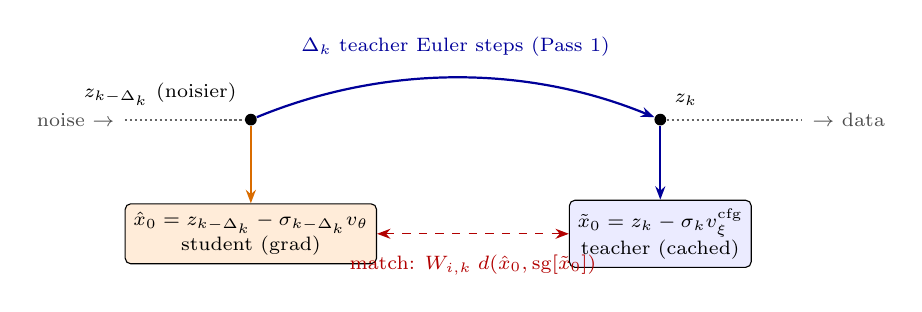
\begin{tikzpicture}[font=\scriptsize,
    pbox/.style={draw, rounded corners=2pt, align=center, inner sep=3pt},
    arr/.style={-{Stealth[length=1.7mm]}, thick}]
    \node[circle, fill=black, inner sep=1.5pt,
      label={[label distance=0pt]above left:{$z_{k-\Delta_k}$ (noisier)}}] (za) at (0,0) {};
    \node[circle, fill=black, inner sep=1.5pt,
      label={[label distance=0pt]above right:{$z_k$}}] (zb) at (5.2,0) {};
    \draw[arr, blue!60!black]
      (za) .. controls (1.7,0.7) and (3.5,0.7) ..
      node[above=4pt] {$\Delta_k$ teacher Euler steps (Pass 1)} (zb);
    \draw[densely dotted, thick, black!60] (zb) -- (7.0,0)
      node[right, black!70] {$\to$ data};
    \draw[densely dotted, thick, black!60] (-1.6,0)
      node[left, black!70] {noise $\to$} -- (za);
    \node[pbox, fill=orange!15] (xs) at (0,-1.45)
      {$\xhat = z_{k-\Delta_k} - \sigma_{k-\Delta_k} v_\theta$\\student (grad)};
    \node[pbox, fill=blue!8] (xt) at (5.2,-1.45)
      {$\xtil = z_k - \sigma_k v^{\mathrm{cfg}}_\xi$\\teacher (cached)};
    \draw[arr, orange!85!black] (za) -- (xs);
    \draw[arr, blue!60!black] (zb) -- (xt);
    \draw[{Stealth[length=1.7mm]}-{Stealth[length=1.7mm]}, dashed, red!70!black]
      (xs) -- node[below=4pt] {match: $W_{i,k}\; d(\xhat, \sg[\xtil])$} (xt);
  \end{tikzpicture}
  \end{center}
  \vspace{-0.4em}
  \begin{itemize}
    \item $z_k$ is reached from $z_{k-\Delta_k}$ by teacher Euler steps
      $\Rightarrow$ both estimate the \emph{same} endpoint: consistency
      distillation in $x_0$ space across an asymmetric gap
      ($\Delta =$ LCM's skipping step).
  \end{itemize}
\end{frame}

\begin{frame}{Scoring and Boltzmann weighting}
  Score every student prediction in CLIP space against the \emph{caption}:
  \[
    s_{i,k} = \cossim\big( g_\phi(\xhat^{(i,k)}),\; \ftext \big)
    \qquad \text{(learned CLIPScore proxy)}
  \]
  Importance weights $=$ product of two Boltzmann distributions with energy
  $E = -s$, \textbf{detached}:
  \[
    w^{\mathrm{traj}}_i = \frac{\exp(\bar{s}_i / \tau_N)}{\sum_{i'} \exp(\bar{s}_{i'} / \tau_N)},
    \quad
    w^{\mathrm{step}}_{i,k} = \frac{\exp(s_{i,k} / \tau_K)}{\sum_{k'} \exp(s_{i,k'} / \tau_K)},
    \quad
    W_{i,k} = \sg\big[ w^{\mathrm{traj}}_i \cdot w^{\mathrm{step}}_{i,k} \big]
  \]
  \begin{itemize}
    \item Scores are \textbf{z-scored along each softmax axis}: raw CLIP
      cosines spread only a few hundredths across samples of one prompt, which
      leaves $\mathrm{softmax}(s/\tau)$ near-uniform; z-scoring makes $\tau$ a
      scale-free selectivity knob (checked via logged weight entropies).
    \item \textbf{Why detach?} Gradient through the softmax would reward
      routing mass onto the easiest pairs --- i.e.\ \emph{lowering} $s$
      exactly where matching is hard.
    \item Detached, $W$ is a self-normalized reward-weighted-regression
      weight \litref{RWR --- Peters \& Schaal, 2007}: a \alert{soft
      best-of-$N$} over trajectories \emph{and} timesteps --- the same
      structure as best-of-$N$ distillation against an EMA anchor in LLM
      alignment. \litref{BOND --- Sessa et al., 2024}
  \end{itemize}
\end{frame}

\begin{frame}{Objective}
  \small
  \[
  \boxed{\;
  \mathcal{L} =
  \underbrace{\sum_{i,k} W_{i,k}\;
    d\big( \xhat^{(i,k)},\, \sg[\xtil^{(i,k)}] \big)}_{\mathcal{L}_{\mathrm{cons}}\;\text{(weighted consistency)}}
  \;+\; \lambda_r
  \underbrace{\frac{1}{N |\mathcal{K}|} \sum_{i,k} \big( 1 - s_{i,k} \big)}_{\mathcal{L}_{\mathrm{reward}}\;\text{(alignment reward)}}
  \;+\; \lambda_a
  \underbrace{\Big( 1 - \cossim\big( g_\phi(\mathcal{E}(x_{\mathrm{real}})),\, \fimg \big) \Big)}_{\mathcal{L}_{\mathrm{align}}\;\text{(projector anchor)}}
  \;}
  \]
  \normalsize
  \begin{itemize}
    \item $\mathcal{L}_{\mathrm{cons}}$: dimension-scaled pseudo-Huber (iCT),
      $d(a,b) = \sqrt{\lVert a - b \rVert_2^2 + c^2} - c$ with
      $c = 0.00054\sqrt{D} \approx 0.14$ --- robust to outliers from
      aggressive gaps.
    \item $\mathcal{L}_{\mathrm{reward}}$: the \emph{only} path through which
      the score reaches the student (ReFL-style, via the cheap projector
      proxy): $\mathcal{L}_{\mathrm{reward}} \to s \to g_\phi(\xhat) \to v_\theta$.
    \item $\mathcal{L}_{\mathrm{align}}$: anchors $g_\phi$ on real-image
      latents; the student receives no gradient from it.
  \end{itemize}
  After each AdamW step: $\xi \leftarrow m\,\xi + (1-m)\,\theta$ (fp32 EMA).
\end{frame}

\begin{frame}{Why these choices}
  \begin{itemize}
    \item \textbf{Consistency in $x_0$ space, not feature space} ---
      $\xhat$ has a fixed meaning at every timestep: no constant-feature
      collapse mode, and the full network sits in the gradient path.
    \item \textbf{Asymmetric gap direction} --- noisier student matching a
      cleaner target along the same trajectory mirrors consistency
      distillation's adjacent-pair structure; transfers late-trajectory
      information to earlier timesteps.
    \item \textbf{CFG-mixed Tweedie targets} --- adherence is distilled into a
      single conditional forward; CFG distillation is implicit RLHF.
      \litref{Luo, 2024}
    \item \textbf{Text-embedding scoring} --- $s$ approximates CLIPScore, the
      actual alignment quantity; scoring against the paired \emph{image}
      embedding would impose single-image reconstruction (captions are
      many-to-many).
    \item \textbf{fp32 masters $+$ fp32 EMA} --- with $m = 0.999$, EMA
      increments are ${\sim}10^{-3}(\theta - \xi)$, below bf16 resolution;
      compute runs under bf16 autocast.
    \item \textbf{Tracked limitations} --- (i) anchor trains on clean latents
      but scores Tweedie predictions (domain gap); (ii) no real-data term for
      the \emph{student}: drift is monitored via periodic EMA samples ---
      the known cost of leaving DMD-style data terms out.
      \litref{cf.\ DMD2 --- Yin et al., 2024}
  \end{itemize}
\end{frame}

\begin{frame}{Setup}
  \begin{center}
  \scriptsize
  \begin{adjustbox}{max width=\textwidth}
  \begin{tabular}{@{}lll@{}}
    \toprule
    \textbf{Component} & \textbf{Value} & \textbf{Notes} \\
    \midrule
    Base model & SD3.5-Medium (2.5B MMDiT) & flow matching, velocity prediction \\
    Encoder & CLIP ViT-L/14 & joint-space embeddings, $d = 768$ \\
    Data & COCO \texttt{train2017} & 591{,}753 (image, caption) pairs; $\fimg$ cached once \\
    Trajectories & $N = 4$, $K = 8$ Euler steps & CFG $\omega = 7.0$ (batched uncond $\Vert$ cond) \\
    Scoring window & $[0.4, 0.9] \cdot K \Rightarrow k \in \{3, \dots, 7\}$ & mid-to-late noise band \\
    Timestep gap & $\Delta \sim \mathcal{U}\{1, 3\}$, one per $k$ & student always noisier than target \\
    Temperatures & $\tau_N = \tau_K = 1.0$, z-scored $s$ & max traj.\ weight ${\approx}0.5$ at $N{=}4$ \\
    Loss weights & $\lambda_r = 1.0$, $\lambda_a = 1.0$ & pseudo-Huber $c \approx 0.14$ (MSE as ablation) \\
    EMA / precision & $m = 0.999$, fp32 masters & bf16 autocast compute \\
    Optimizer & AdamW; LR $10^{-5}$ (student), $10^{-4}$ (projector) & warmup 500; grad clip 1.0 / 5.0 \\
    Batching & 1 caption/rank/step; pass 2 $= 20$-forward & gradient checkpointing \\
    Hardware & $4 \times$ H200 (141 GB), DDP & rank-disjoint prompt streams; 150k steps \\
    \bottomrule
  \end{tabular}
  \end{adjustbox}
  \end{center}
\end{frame}

% ===========================================================================
\section{Evaluation, ablations, and risks}
% ===========================================================================

\begin{frame}{Core ablations to make the claim credible}
  \scriptsize
  \begin{center}
  \begin{adjustbox}{max width=\textwidth}
  \begin{tabular}{@{}p{0.24\textwidth}p{0.34\textwidth}p{0.32\textwidth}@{}}
    \toprule
    \textbf{Ablation} & \textbf{Question answered} & \textbf{Expected diagnostic} \\
    \midrule
    Uniform \(W\), no scorer & Is consistency self-distillation alone responsible? & isolates distillation from alignment weighting \\
    Keep scorer, remove \(\mathcal{L}_{\mathrm{reward}}\) & Do weights alone help without direct reward gradient? & tests selection-only vs reward-gradient contribution \\
    Keep reward, uniform \(W\) & Is the effect from reward fine-tuning rather than target selection? & separates ReFL-like term from weighted consistency \\
    No image-feature anchor & Does projector collapse or reward hacking appear? & watch \(\|g_\phi\|\), score entropy, external CLIPScore \\
    Text scorer vs image scorer & Does scoring against captions preserve many-to-many caption semantics? & image scorer should overfit paired image semantics \\
    No CFG-mixed target / lower CFG & Is guidance being distilled into the weights? & should reduce prompt adherence if CFG is key \\
    Vary \(N,K,\Delta,\tau\) & Is best-of-\(N\) selection or temporal selection doing the work? & entropy and metric curves should change predictably \\
    \bottomrule
  \end{tabular}
  \end{adjustbox}
  \end{center}
\end{frame}

\begin{frame}{Concrete baselines from the literature}
  \begin{itemize}
    \item \textbf{Uniform latent matching}: same EMA teacher, same $x_0$
      consistency, but $W_{i,k}=1/(N|\mathcal{K}|)$ and no reward term ---
      the headline ablation (\texttt{--latent\_matching\_baseline}).
    \item \textbf{LCM-style weighting}: same gaps but no trajectory-level
      best-of-$N$; isolates whether scoring or just asymmetric gaps help.
    \item \textbf{Reward-only vs weighted consistency}: remove
      $\mathcal{L}_{\mathrm{reward}}$ \emph{or} remove the score-dependent $W$
      to separate gradient signal from data-selection signal.
    \item \textbf{Projector anchor ablation}: remove $\mathcal{L}_{\mathrm{align}}$
      to test for reward hacking / score collapse.
    \item \textbf{External references}: SD3.5-M base, CFG-only at matched NFE,
      LCM / SD3.5-Flash few-step, and (compute permitting) a ReFL-style
      reward-FT baseline.
  \end{itemize}
\end{frame}

\begin{frame}{Evaluation protocol}
  \footnotesize
  \begin{itemize}
    \item \textbf{Primary alignment}: CLIPScore on COCO captions;
      T2I-CompBench overall and per split (color, shape, texture, spatial,
      non-spatial, complex); GenEval object-focused score.
    \item \textbf{Quality / diversity guardrails}: COCO FID/KID; aesthetic
      score if available; diversity across seeds; VAE latent variance;
      negative-prompt stress tests.
    \item \textbf{Efficiency}: NFEs, wall-clock latency, VRAM, and whether
      CFG is needed at inference.
    \item \textbf{Training health}: score distribution, trajectory/step
      entropies, projector anchor cosine, external decoded CLIPScore
      correlation with the latent proxy, EMA sample drift.
    \item \textbf{Human check}: blind side-by-side preference on a small,
      balanced prompt set --- COCO easy captions, T2I-CompBench binding
      prompts, counting/spatial prompts, and adversarial long prompts.
  \end{itemize}
  \begin{block}{Recommended minimum package}
    COCO FID/KID $+$ CLIPScore for generic quality/alignment; T2I-CompBench
    and GenEval for composition; side-by-side human preference for the
    quality/adherence trade-off.
  \end{block}
\end{frame}

\begin{frame}{Failure modes to actively rule out}
  \footnotesize
  \begin{itemize}
    \item \textbf{Proxy over-optimization}: latent scorer rises, but decoded
      images become lower quality or exploit CLIP shortcuts.
    \item \textbf{Projector collapse}: \(g_\phi\) learns text-aligned
      directions that no longer behave like image embeddings; anchor loss and
      external CLIP correlation should catch this.
    \item \textbf{Mode narrowing}: soft best-of-\(N\) can favor common, simple
      completions; monitor diversity and seed sensitivity.
    \item \textbf{Temporal bias}: mid/late windows may ignore early global
      layout errors; test wider/narrower scoring windows.
    \item \textbf{Self-distillation feedback loop}: EMA teacher inherits
      student artifacts; periodically compare to the frozen base teacher on
      fixed prompts.
    \item \textbf{Compositional blind spots}: CLIP-style global cosine may
      miss swapping/binding; GenEval and T2I-CompBench are required before
      claiming prompt-adherence gains.
  \end{itemize}
\end{frame}

\begin{frame}{Research risks made visible by the literature}
  \begin{itemize}
    \item \textbf{Reward hacking}: ReFL / AlignProp / ReNO show reward
      optimization finds shortcuts; our projector anchor and detached weights
      reduce but do not eliminate this. \litref{Clark et al., 2024; Eyring et al., 2024}
    \item \textbf{Teacher-path overfitting}: PD and LCM inherit teacher path
      biases; soft best-of-$N$ may reduce bad target mass, but still learns
      from teacher trajectories.
    \item \textbf{Large-skip instability}: consistency / flow-map papers show
      quality degrades under aggressive jumps; our gap distribution and
      pseudo-Huber loss are safeguards. \litref{Sabour et al., 2025}
    \item \textbf{Metric mismatch}: CLIPScore correlates with compatibility
      but is imperfect for compositional semantics; T2I-CompBench / GenEval /
      human eval are necessary downstream checks.
    \item \textbf{Flow-matching transfer}: SiD-DiT and AYF make transfer to
      SD3.5-style FM models plausible, but the alignment-weighted objective is
      still the novel, unvalidated part.
  \end{itemize}
\end{frame}

% ===========================================================================
\section{Early results}
% ===========================================================================

\begin{frame}{What we monitor (wandb)}
  \begin{itemize}
    \item \textbf{Alignment} --- \texttt{train/s\_mean} (learned CLIPScore
      proxy; want $\uparrow$), \texttt{s\_std} / \texttt{s\_min} /
      \texttt{s\_max}, \texttt{train/L\_reward}.
    \item \textbf{Selectivity} --- \texttt{train/w\_traj\_entropy}
      ($\le \ln N$), \texttt{train/w\_step\_entropy}
      ($\le \ln |\mathcal{K}|$), \texttt{train/W\_entropy}: pinned at the
      maximum $\Rightarrow$ the weighting is inert.
    \item \textbf{Projector health} --- \texttt{train/L\_align},
      \texttt{train/align\_cos} ($\uparrow$), output / parameter L2 norms,
      projector vs.\ student grad norms (clipped separately).
    \item \textbf{Distillation} --- \texttt{train/d\_mean} (weighted
      consistency), grad-norm / clip ratio, $\sigma$ levels,
      \texttt{train/avg\_delta}.
    \item \textbf{Qualitative} --- \texttt{samples/teacher\_ema}: EMA-teacher
      samples every 500 steps on 4 COCO $+$ 4 T2I-CompBench prompts.
    \item \textbf{Baseline} --- \texttt{--latent\_matching\_baseline}: uniform
      $W$, no scoring --- isolates the contribution of encoder-scored
      weighting.
  \end{itemize}
\end{frame}

\begin{frame}{Early results --- live in wandb}
  % Drop screenshots in later, e.g.:
  %   \includegraphics[width=0.48\textwidth]{figs/wandb_curves.png}
  %   \includegraphics[width=0.48\textwidth]{figs/wandb_samples.png}
  \begin{columns}[T]
    \begin{column}{0.48\textwidth}
      \centering
      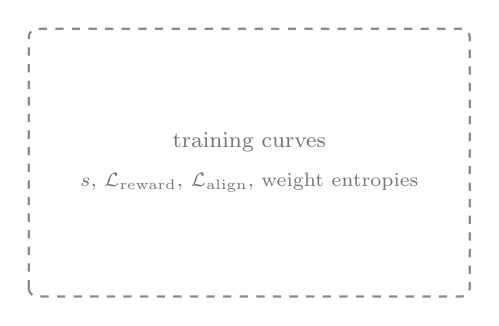
\begin{tikzpicture}
        \draw[dashed, thick, black!45, rounded corners=3pt] (0,0) rectangle (5.6,3.4);
        \node[align=center, black!55] at (2.8,1.7)
          {\footnotesize training curves\\[2pt]\scriptsize
           $s$, $\mathcal{L}_{\mathrm{reward}}$, $\mathcal{L}_{\mathrm{align}}$,
           weight entropies};
      \end{tikzpicture}
    \end{column}
    \begin{column}{0.48\textwidth}
      \centering
      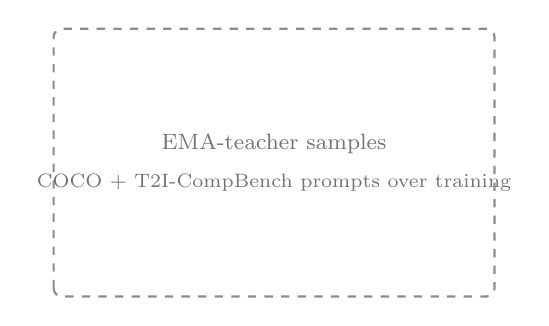
\begin{tikzpicture}
        \draw[dashed, thick, black!45, rounded corners=3pt] (0,0) rectangle (5.6,3.4);
        \node[align=center, black!55] at (2.8,1.7)
          {\footnotesize EMA-teacher samples\\[2pt]\scriptsize
           COCO $+$ T2I-CompBench prompts over training};
      \end{tikzpicture}
    \end{column}
  \end{columns}
  \vspace{1.0em}
  \begin{center}
    $\rightarrow$ \alert{live wandb dashboard}
  \end{center}
\end{frame}

% ===========================================================================
% APPENDIX --- backup tables, annotated bibliography, full reference list
% (merged from all three source decks; references checked June 2026)
% ===========================================================================
\appendix

\section{Backup: maps of the literature}

\begin{frame}{Backup --- map of the prior-work space}
  \scriptsize
  \begin{center}
  \begin{adjustbox}{max width=\textwidth}
  \begin{tabular}{@{}L{0.18\textwidth}L{0.23\textwidth}L{0.25\textwidth}L{0.24\textwidth}@{}}
    \toprule
    \textbf{Family} & \textbf{Signal / teacher} & \textbf{What is matched} & \textbf{Why it matters here} \\
    \midrule
    Diffusion foundations & DDPM, score SDE, DDIM, CFG & score / noise / \(x_0\); PF-ODE path & establishes the ODE and guidance objects we distill \\
    Trajectory distillation & frozen diffusion sampler & one or two teacher steps, often DDIM & gives pairwise teacher--student targets \\
    Consistency / flow maps & PF-ODE trajectories & endpoint \(f(x_t,t)\) or jump \(t \to s\) & nearest ancestor of our asymmetric gap loss \\
    Distribution / score distill & frozen score model, discriminator & output distribution, score identity, adversarial realism & closest alternative when one-to-one trajectory matching is avoided \\
    Flow matching distill & rectified / FM teacher & shortcut / average velocity / continuous flow map & most related to SD3.5-Medium as a flow-matching DiT \\
    Reward / preference align & reward model or preference pairs & high-reward samples / gradients / DPO loss & alignment axis; usually pays decode $+$ reward cost \\
    Representation alignment & CLIP / DINO / DINOv2 encoders & hidden features or latent-to-feature regression & gives the latent scorer and projector idea \\
    \bottomrule
  \end{tabular}
  \end{adjustbox}
  \end{center}
  \vspace{0.3em}
  \begin{alertblock}{Literature gap}
    Prior work either distills for speed, or fine-tunes for reward/preference
    alignment. The closest open gap is \emph{using distillation rollouts
    themselves as an encoder-scored selection mechanism for prompt adherence
    in a flow-matching T2I model}.
  \end{alertblock}
\end{frame}

\begin{frame}{Backup --- foundations: diffusion, PF-ODEs, flow matching}
  \scriptsize
  \begin{center}
  \begin{adjustbox}{max width=\textwidth}
  \begin{tabular}{@{}L{0.22\textwidth}L{0.33\textwidth}L{0.35\textwidth}@{}}
    \toprule
    \textbf{Work} & \textbf{Core idea} & \textbf{Takeaway for this project} \\
    \midrule
    DDPM \litref{Ho et al., 2020} & learns denoising transitions / score-related noise prediction; high quality but many steps & sampling cost motivates distillation \\
    Score SDE / PF-ODE \litref{Song et al., 2021} & reverse SDE has an equivalent probability-flow ODE with the same marginals & defines the deterministic trajectory consistency distillation uses \\
    DDIM \litref{Song et al., 2021} & non-Markovian reverse process with faster deterministic sampling & common teacher path for progressive distillation \\
    CFG \litref{Ho \& Salimans, 2022} & mixes conditional and unconditional predictions to trade diversity for fidelity/adherence & doubles NFE; guided distillation can absorb this cost into one conditional model \\
    Flow Matching \litref{Lipman et al., 2023} & simulation-free regression of vector fields for conditional probability paths & SD3-style models are naturally described as velocity / flow fields \\
    Rectified Flow \litref{Liu et al., 2023} & learn ODEs following straight paths; reflow can straighten couplings & few-step flow distillation is often about shortening / straightening the path \\
    Stochastic Interpolants \litref{Albergo et al., 2023} & unifies flows and diffusions through flexible stochastic bridges & supports viewing diffusion/FM distillation as flow-map learning \\
    \bottomrule
  \end{tabular}
  \end{adjustbox}
  \end{center}
\end{frame}

% ---------------------------------------------------------------------------
\section{Backup: annotated bibliography}

\begin{frame}[shrink=6]{Annotated bibliography I --- trajectory and consistency}
  \scriptsize
  \begin{adjustbox}{max width=\textwidth, max height=0.80\textheight, center}
  \begin{tabular}{@{}L{0.22\textwidth}L{0.34\textwidth}L{0.34\textwidth}@{}}
    \toprule
    \textbf{Paper} & \textbf{Core contribution} & \textbf{Use in our argument} \\
    \midrule
    Luhman \& Luhman, 2021 & Directly train a student to map noise to a teacher sample, avoiding iterative sampling. & Historical endpoint-regression baseline; illustrates cost of offline targets. \\
    Salimans \& Ho, 2022 & Progressive distillation: one student step matches two DDIM teacher steps; repeat halving. & Canonical trajectory-distillation recipe; motivates matching teacher endpoint estimates. \\
    Song et al., 2023 & Consistency models learn an endpoint map invariant along PF-ODE trajectories. & Provides the core self-consistency principle. \\
    Song \& Dhariwal, 2024 & Improved consistency training with pseudo-Huber losses and curriculum choices. & Direct source for our robust pseudo-Huber metric. \\
    Luo et al., 2023 & Latent Consistency Models distill guided latent diffusion for 1--4 step T2I. & Closest architecture-level precedent for guided latent consistency. \\
    Zheng et al., 2024 & TCD improves LCM through trajectory mapping and stochastic sampling. & Supports our concern about skip/gap error and trajectory structure. \\
    Kim et al., 2024 & CTM learns arbitrary transitions along the PF-ODE and recovers speed--quality tradeoffs. & Bridges endpoint consistency to richer flow-map objectives. \\
    \bottomrule
  \end{tabular}
  \end{adjustbox}
\end{frame}

\begin{frame}[shrink=6]{Annotated bibliography II --- flow matching and flow maps}
  \scriptsize
  \begin{adjustbox}{max width=\textwidth, max height=0.80\textheight, center}
  \begin{tabular}{@{}L{0.22\textwidth}L{0.34\textwidth}L{0.34\textwidth}@{}}
    \toprule
    \textbf{Paper} & \textbf{Core contribution} & \textbf{Use in our argument} \\
    \midrule
    Liu et al., 2024 / InstaFlow & Applies rectified-flow distillation/reflow to one-step T2I generation. & Early evidence that flow/rectified-flow acceleration can work for T2I. \\
    Boffi et al., 2024 / FMM & Formalizes flow-map matching for two-time maps under stochastic interpolants. & Mathematical foundation for consistency-style jumps. \\
    Boffi et al., 2025 / self-distill & Builds consistency models by learning flow maps via self-distillation. & Names the self-distillation mechanism we adopt for the gap loss. \\
    Frans et al., 2025 / Shortcut & Adds desired step-size conditioning so one model works across step budgets. & Alternative to explicit progressive distillation schedules. \\
    Geng et al., 2025 / MeanFlow & Models average velocity for strong one-step generation from scratch. & Shows average/jump quantities can be more natural than instantaneous velocity. \\
    Sabour et al., 2025 / AYF & Scales continuous-time flow-map distillation; text-to-image few-step results. & Closest modern flow-map distillation line. \\
    Chen et al., 2025 / SANA-Sprint & Hybrid distillation for 1--4 step SANA flow-matching T2I. & Practical FM foundation-model distillation example. \\
    \bottomrule
  \end{tabular}
  \end{adjustbox}
\end{frame}

\begin{frame}[shrink=6]{Annotated bibliography III --- distribution, adversarial, score}
  \scriptsize
  \begin{adjustbox}{max width=\textwidth, max height=0.78\textheight, center}
  \begin{tabular}{@{}L{0.22\textwidth}L{0.34\textwidth}L{0.34\textwidth}@{}}
    \toprule
    \textbf{Paper} & \textbf{Core contribution} & \textbf{Use in our argument} \\
    \midrule
    Sauer et al., 2024 / ADD & Combines score distillation and adversarial loss; powers SDXL-Turbo-like low-step generation. & Shows few-step fidelity often needs non-$\ell_2$ objectives. \\
    Yin et al., 2024a / DMD & Matches generated and teacher output distributions by score-function differences. & Alternative to pairwise trajectory imitation. \\
    Yin et al., 2024b / DMD2 & Stabilizes DMD, removes expensive regression-pair construction, adds GAN term. & Useful baseline for few-step quality/fidelity and critic-based training. \\
    Zhou et al., 2024 / SiD & Data-free score identity distillation for one-step diffusion generation. & Closest score-theoretic distillation approach. \\
    Zhou et al., 2025 / SiD-DiT & Extends score identity distillation to SANA, SD3/3.5, and FLUX. & Direct evidence that SD3.5-style flow-matching DiTs can be distilled. \\
    Dao et al., 2025 / SCFlow & Self-corrected flow distillation combines consistency and adversarial training. & Recent evidence for multi-objective flow distillation. \\
    \bottomrule
  \end{tabular}
  \end{adjustbox}
\end{frame}

\begin{frame}[shrink=6]{Annotated bibliography IV --- reward and preference alignment}
  \scriptsize
  \begin{adjustbox}{max width=\textwidth, max height=0.80\textheight, center}
  \begin{tabular}{@{}L{0.22\textwidth}L{0.34\textwidth}L{0.34\textwidth}@{}}
    \toprule
    \textbf{Paper} & \textbf{Core contribution} & \textbf{Use in our argument} \\
    \midrule
    Xu et al., 2023 / ImageReward $+$ ReFL & Human-preference reward model plus reward-feedback learning for T2I diffusion. & Main reward-model baseline and motivation for avoiding decoded reward calls. \\
    Black et al., 2024 / DDPO & Treats denoising as an RL process and optimizes downstream reward via policy gradients. & Shows reward optimization can improve alignment but is compute-heavy. \\
    Prabhudesai et al., 2024 / AlignProp & Backpropagates differentiable rewards through denoising using LoRA/checkpointing. & Closest direct reward-gradient route. \\
    Kirstain et al., 2023 / Pick-a-Pic & Public human preference dataset and PickScore reward model. & Preference data source used by alignment baselines. \\
    Wallace et al., 2024 / Diffusion-DPO & DPO-style preference optimization for diffusion likelihoods; improves SDXL preference/alignment. & Closest preference-learning baseline; contrasts with no human pairs in our loop. \\
    Eyring et al., 2024 / ReNO & Optimizes initial noise of one-step T2I models at inference with reward gradients. & Related to best-of/noise selection but happens at inference, not training. \\
    \bottomrule
  \end{tabular}
  \end{adjustbox}
\end{frame}

\begin{frame}[shrink=6]{Annotated bibliography V --- representations and evaluation}
  \scriptsize
  \begin{adjustbox}{max width=\textwidth, max height=0.80\textheight, center}
  \begin{tabular}{@{}L{0.22\textwidth}L{0.34\textwidth}L{0.34\textwidth}@{}}
    \toprule
    \textbf{Paper} & \textbf{Core contribution} & \textbf{Use in our argument} \\
    \midrule
    Hessel et al., 2021 / CLIPScore & Uses CLIP image--text cosine as a reference-free compatibility metric. & Defines the score proxy we amortize in latent space. \\
    Huang et al., 2023 / T2I-CompBench & Benchmark for compositional T2I: attribute binding, relations, complex prompts. & Main evaluation target for alignment gains. \\
    Oquab et al., 2023 / DINOv2 & Strong frozen visual foundation features from self-supervised training. & Motivates frozen encoder feature spaces as useful training signals. \\
    Yu et al., 2025 / REPA & Aligns DiT hidden states to frozen visual representations via a lightweight projector. & Direct inspiration for projector-based representation supervision. \\
    Radford et al., 2021 / CLIP & Joint text--image contrastive representation. & Provides the shared semantic space for our scorer. \\
    \bottomrule
  \end{tabular}
  \end{adjustbox}
\end{frame}

\begin{frame}[shrink=6]{Backup --- recommended baselines and ablations}
  \footnotesize
  \begin{itemize}
    \item \textbf{Uniform latent matching}: same EMA teacher, same $x_0$
      consistency, but $W_{i,k}=1/(N|\mathcal{K}|)$ and no reward term.
    \item \textbf{LCM-style weighting}: same gaps but no trajectory-level
      best-of-$N$; isolates whether scoring or just asymmetric gaps help.
    \item \textbf{Reward only vs.\ weighted consistency}: remove
      $\mathcal{L}_{\mathrm{reward}}$ or remove the score-dependent $W$ to
      separate the gradient signal from the data-selection signal.
    \item \textbf{Projector anchor ablation}: remove
      $\mathcal{L}_{\mathrm{align}}$ to test for reward hacking / score
      collapse.
    \item \textbf{Metric checks}: learned proxy score, decoded CLIPScore,
      ImageReward/PickScore, T2I-CompBench, GenEval, and human side-by-side.
  \end{itemize}
\end{frame}

% ---------------------------------------------------------------------------
\section{Full reference list}

\begin{frame}[allowframebreaks]{References (checked June 2026)}
  \scriptsize
  \textbf{Solvers \& foundations}
  \begin{itemize}
    \item Ho, Jain, Abbeel. \emph{Denoising Diffusion Probabilistic Models.} NeurIPS 2020.
    \item Song, Sohl-Dickstein, Kingma, Kumar, Ermon, Poole. \emph{Score-Based Generative Modeling through SDEs.} ICLR 2021.
    \item Song, Meng, Ermon. \emph{Denoising Diffusion Implicit Models (DDIM).} ICLR 2021.
    \item Lu et al. \emph{DPM-Solver: A Fast ODE Solver for Diffusion Probabilistic Model Sampling.} NeurIPS 2022.
    \item Karras, Aittala, Aila, Laine. \emph{Elucidating the Design Space of Diffusion-Based Generative Models (EDM).} NeurIPS 2022.
    \item Ho \& Salimans. \emph{Classifier-Free Diffusion Guidance.} arXiv:2207.12598, 2022.
    \item Lipman et al. \emph{Flow Matching for Generative Modeling.} ICLR 2023. \quad Liu, Gong, Liu. \emph{Flow Straight and Fast (Rectified Flow).} ICLR 2023.
    \item Esser et al. \emph{Scaling Rectified Flow Transformers for High-Resolution Image Synthesis (SD3 / MMDiT).} ICML 2024.
    \item Albergo et al. \emph{Stochastic Interpolants.} 2023. \quad Kingma \& Gao. NeurIPS 2023. \quad Gao et al. \emph{Diffusion Meets Flow Matching.} 2024.
  \end{itemize}
  \textbf{Trajectory \& consistency distillation}
  \begin{itemize}
    \item Luhman \& Luhman. \emph{Knowledge Distillation in Iterative Generative Models.} arXiv:2101.02388, 2021.
    \item Salimans \& Ho. \emph{Progressive Distillation for Fast Sampling of Diffusion Models.} ICLR 2022.
    \item Meng et al. \emph{On Distillation of Guided Diffusion Models.} CVPR 2023. \quad Gu et al. \emph{BOOT.} 2023.
    \item Liu et al. \emph{InstaFlow.} ICLR 2024. \quad Wang et al. \emph{Rectified Diffusion.} 2025.
    \item Song, Dhariwal, Chen, Sutskever. \emph{Consistency Models.} ICML 2023.
    \item Song \& Dhariwal. \emph{Improved Techniques for Training Consistency Models (iCT).} ICLR 2024.
    \item Luo et al. \emph{Latent Consistency Models.} arXiv:2310.04378, 2023. \quad Wang et al. \emph{Phased Consistency Models.} NeurIPS 2024.
    \item Kim, Lai, Liao, Murata, Takida, Uesaka, He, Mitsufuji, Ermon. \emph{Consistency Trajectory Models.} ICLR 2024.
    \item Lu \& Song. \emph{Simplifying, Stabilizing and Scaling Continuous-Time Consistency Models (sCM / TrigFlow).} ICLR 2025.
    \item Zheng et al. \emph{Trajectory Consistency Distillation (TCD).} 2024. \quad Ren et al. \emph{Hyper-SD.} NeurIPS 2024.
    \item Lin, Wang, Yang. \emph{SDXL-Lightning: Progressive Adversarial Diffusion Distillation.} 2024. \quad Chadebec et al. \emph{Flash Diffusion.} 2024.
    \item Chen et al. \emph{SANA-Sprint.} 2025.
    \item Zheng et al. \emph{Large-Scale Diffusion Distillation via Score-Regularized Continuous-Time Consistency (rCM).} arXiv:2510.08431, 2025.
  \end{itemize}
  \textbf{Flow maps}
  \begin{itemize}
    \item Boffi, Albergo, Vanden-Eijnden. \emph{Flow Map Matching.} arXiv:2406.07507, TMLR 2025.
    \item Boffi, Albergo, Vanden-Eijnden. \emph{How to Build a Consistency Model: Learning Flow Maps via Self-Distillation.} arXiv:2505.18825, NeurIPS 2025.
    \item Frans, Hafner, Levine, Abbeel. \emph{One Step Diffusion via Shortcut Models.} ICLR 2025.
    \item Geng, Deng, Bai, Kolter, He. \emph{Mean Flows for One-Step Generative Modeling.} NeurIPS 2025 (oral).
    \item Sabour, Fidler, Kreis. \emph{Align Your Flow: Scaling Continuous-Time Flow Map Distillation.} arXiv:2506.14603, NeurIPS 2025.
    \item Ai et al. \emph{Joint Distillation for Fast Likelihood Evaluation and Sampling in Flow-Based Models (F2D2).} arXiv:2512.02636, ICLR 2026.
  \end{itemize}
  \textbf{Score / distribution distillation}
  \begin{itemize}
    \item Poole, Jain, Barron, Mildenhall. \emph{DreamFusion (SDS).} ICLR 2023. \quad Wang et al. \emph{ProlificDreamer (VSD).} NeurIPS 2023.
    \item Luo et al. \emph{Diff-Instruct.} NeurIPS 2023. \quad Nguyen \& Tran. \emph{SwiftBrush.} CVPR 2024.
    \item Yin et al. \emph{One-Step Diffusion with Distribution Matching Distillation (DMD).} CVPR 2024.
    \item Yin et al. \emph{Improved Distribution Matching Distillation (DMD2).} NeurIPS 2024 (oral).
    \item Zhou, Zheng, Wang, Yin, Huang. \emph{Score Identity Distillation (SiD).} ICML 2024; \emph{SiD-LSG} ICLR 2025; \emph{SiDA} ICLR 2025; \emph{Few-Step SiD} arXiv:2505.12674.
    \item Zhou, Gu, Zheng, Song, He, Zhang, Hu, Yang. \emph{Score Distillation of Flow Matching Models (SiD-DiT).} arXiv:2509.25127, 2025.
    \item Xu et al. \emph{$f$-Distill.} 2025. \quad Huang, Geng, Luo, Qi. \emph{Flow Generator Matching.} arXiv:2410.19310, 2024.
    \item Sauer et al. \emph{Adversarial Diffusion Distillation (ADD / SDXL-Turbo).} 2023; \emph{LADD (SD3-Turbo).} 2024.
    \item Dao et al. \emph{Self-Corrected Flow Distillation (SCFlow).} 2025.
    \item Bandyopadhyay et al. \emph{SD3.5-Flash: Distribution-Guided Distillation of Generative Flows.} arXiv:2509.21318, 2025.
    \item Fan, Wu, Wu. \emph{A Survey on Pre-trained Diffusion Model Distillations.} arXiv:2502.08364, 2025.
  \end{itemize}
  \textbf{Alignment, rewards, RL, selection}
  \begin{itemize}
    \item Hessel et al. \emph{CLIPScore.} EMNLP 2021. \quad Huang et al. \emph{T2I-CompBench (incl.\ GORS).} NeurIPS 2023. \quad Ghosh et al. \emph{GenEval.} NeurIPS 2023 D\&B.
    \item Xu et al. \emph{ImageReward $+$ ReFL.} NeurIPS 2023. \quad Wu et al. \emph{HPSv2.} 2023. \quad Kirstain et al. \emph{Pick-a-Pic / PickScore.} NeurIPS 2023.
    \item Black et al. \emph{DDPO.} ICLR 2024. \quad Fan et al. \emph{DPOK.} NeurIPS 2023.
    \item Clark et al. \emph{DRaFT.} ICLR 2024. \quad Prabhudesai et al. \emph{AlignProp.} ICLR 2024.
    \item Wallace et al. \emph{Diffusion-DPO.} CVPR 2024. \quad Eyring et al. \emph{ReNO: Reward-based Noise Optimization.} arXiv:2406.04312, 2024.
    \item Liu et al. \emph{Flow-GRPO: Training Flow Matching Models via Online RL.} NeurIPS 2025.
    \item Xue et al. \emph{DanceGRPO.} arXiv:2505.07818, 2025.
    \item Peters \& Schaal. \emph{Reinforcement Learning by Reward-Weighted Regression.} ICML 2007. \quad Dong et al. \emph{RAFT.} TMLR 2023.
    \item Ma et al. \emph{Inference-Time Scaling for Diffusion Models beyond Scaling Denoising Steps.} arXiv:2501.09732, 2025.
    \item Sessa et al. \emph{BOND: Aligning LLMs with Best-of-$N$ Distillation.} arXiv:2407.14622, 2024.
  \end{itemize}
  \textbf{Reward-aware distillation \& representation alignment}
  \begin{itemize}
    \item Li, Feng, Fu, Wang, Basu, Chen, Wang. \emph{T2V-Turbo.} NeurIPS 2024; \emph{T2V-Turbo-v2.} ICLR 2025.
    \item Li et al. \emph{Reward Guided Latent Consistency Distillation (RG-LCD).} ICLR 2025.
    \item Luo. \emph{Diff-Instruct++: Aligning One-Step Generators with Human Preferences.} arXiv:2410.18881, 2024.
    \item Oquab et al. \emph{DINOv2: Learning Robust Visual Features without Supervision.} 2023/2024.
    \item Yu et al. \emph{Representation Alignment for Generation (REPA).} ICLR 2025.
    \item Leng et al. \emph{REPA-E: Unlocking VAE for End-to-End Tuning of Latent Diffusion Transformers.} ICCV 2025. \quad Tian et al. \emph{U-REPA.} 2025.
    \item Lee, Cha, Kim, Ye. \emph{Aligning Text to Image in Diffusion Models is Easier Than You Think (SoftREPA).} arXiv:2503.08250, 2025.
    \item Radford et al. \emph{Learning Transferable Visual Models from Natural Language Supervision (CLIP).} ICML 2021.
    \item Hu et al. \emph{ELatentLPIPS / latent-space perceptual metrics.} 2024 (latent-space scoring precedent).
  \end{itemize}
\end{frame}

\end{document}
